\section{Analyse og resultater}
Dette afsnit er en undersøgelse af trygheden på Nytorv, som er baseret på observationer af området og interviews af fodgængere. Projektets tilgang til trafikale problemer, vil blive vurderet ud fra disse observationer og interviews. Resultaterne af projektet vil blive præsenteret i dette afsnit, hvoraf der vil blive givet en lille konklusion som afslutning af hver undersøgelse. Afsnittet er altså en sammenkobling af empiri, teori og vurderinger af de forskellige undersøgelser. 


\subsection{Shared Space træk i Nytorv/Østerågade området}
\label{omrade_sharedspace}
For at få en forståelse af hvordan trafikanterne færdes i Nytorv/Østerågade området, er det vigtigt først at fastlægge, hvilken type område det er. Området har mange træk fra Shared Space, og derfor er det relevant at sammenligne området med dette begreb.
Tit og ofte anvender man Shared Space i områder, hvor der er et kryds, eller hvor der er et sammenhængende område, for at skabe en slags balance mellem de forskellige trafikantgrupper. ((en kilde))

\begin{figure}[htbp]
   \label{fig:Nytorv}
   \centering
   \begin{adjustbox}{max width=\textwidth}
     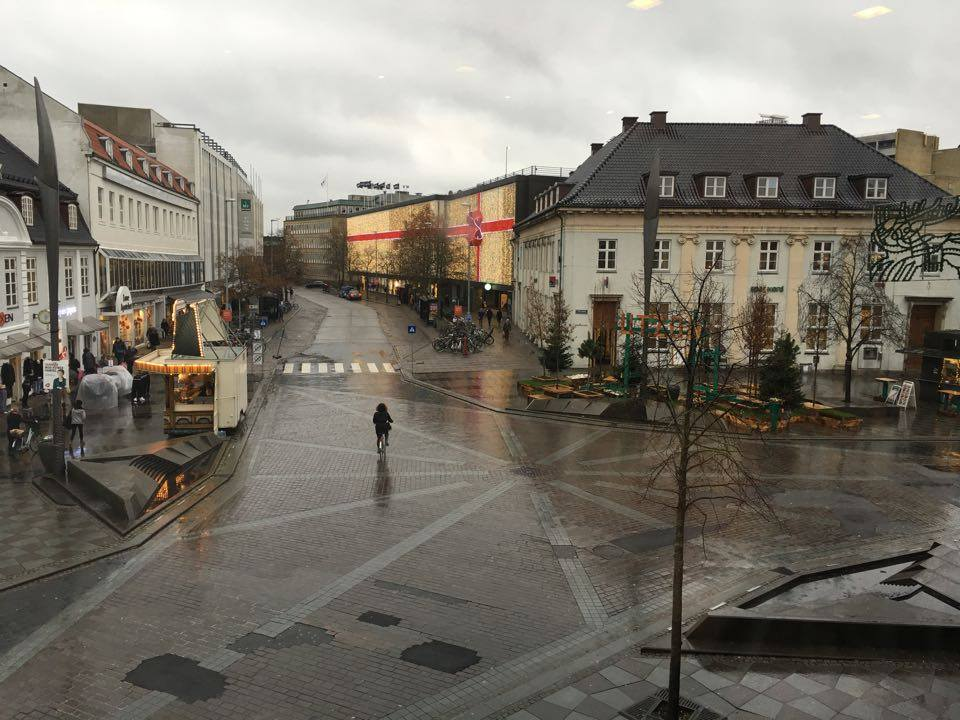
\includegraphics[scale=0.3]{billederogfigur/Nytorvoverblik.jpg}
  \end{adjustbox}
   \caption{Oveblik over Nytorv}
 \end{figure}

Med en balance menes der, at et af formålene med et Shared Space er at ingen af trafikantgrupperne vægtes højere end andre trafikantgrupper. På den måde vil man ikke bryde et sammenhængende område, da man forsøger at kombinere hele områdets funktioner i et. Netop dette princip kan tydeligt fornemmes nede ved Nytorv/Østerågade området. På \cref{fig:Nytorv} kan der ses, at området består af et T-kryds, hvor der rundt om er placeret mange shopping faciliteter og caféer. Desuden forbinder området de to gågader, som gør området til et sammenhængende område. Kriterierne for et område, hvor Shared Space kan benyttes, er altså her opfyldt.
Det er tydeligt, at belægningerne, både på fortov og vej, er meget lig udeseende, hvilket er typisk for et Shared Space område ((kilde)). Der er heller ikke meget afmærkning i form af cykelstier eller kørebaner, som ville have haft til formål at lede trafikanterne. Skiltning, er heller ikke meget brugt og typisk ser man kun et ”E49-, E51- eller E53-skilt” i Shared Space områder, som enten fortæller, om det er en gågade, opholds- og legeområde, eller en fartdæmpet zone, hvor makshastigheden typisk må være 20-30 km/t. Der er altså ikke noget skilt, som decideret er tildelt til Shared Space områder. ((kilde)) Rundt om Nytorv/Østerågade området, er der skiltet med E53-skilte, hvor der er en tilladt makshastighed på 30 km/t. Det kan ses på \cref{fig:Skiltning}, som er taget ved Adelgade, lige inden man kommer ind i Nytorv/Østerågade området.

\begin{figure}[htbp]
   \label{fig:Skiltning}
   \centering
   \begin{adjustbox}{max width=\textwidth}
     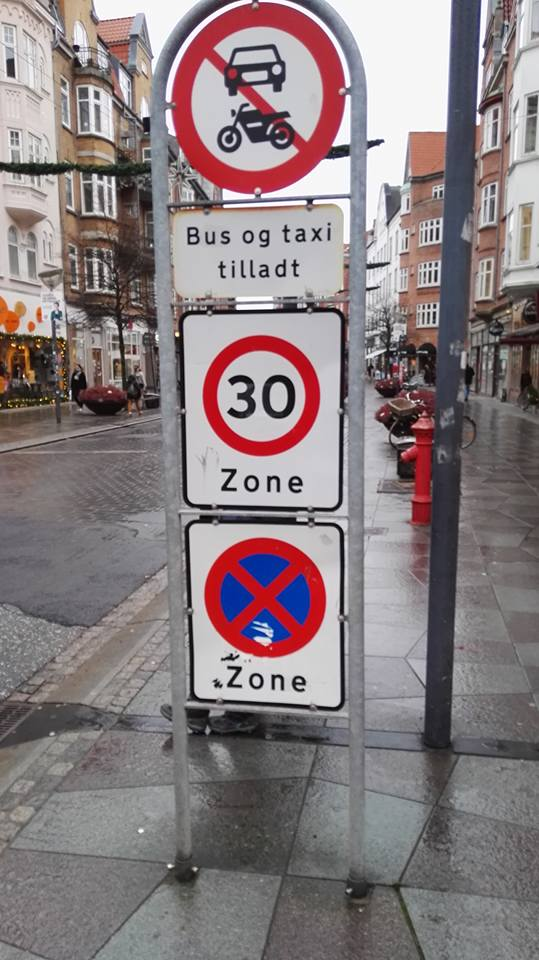
\includegraphics[scale=0.2]{billederogfigur/skiltning.jpg}
  \end{adjustbox}
   \caption{Skiltning rundt om området}
 \end{figure}
\linebreak
I området er der dog en del bustrafik, som ikke anbefales at benytte sig af gennem et Shared Space område. Det er hovedsagligt fordi fokus er på balancen mellem trafikantgrupperne. Busserne vil ofte være nødsaget til at skulle holde tilbage for de mange passerende fodgængere, og det vil kunne forsinke bustrafikken og dermed den kollektive trafik. Dog er der oftest i ruteplanerne taget højde for en sådan forsinkelse, og på korte strækninger vil indflydelsen kunne tænkes at være begrænset. Busserne kræver nogle busstoppesteder, for at passagerer kan stige af og på busserne i området.

\begin{figure}[htbp]
   \label{fig:Busstoppesteder}
   \centering
   \begin{adjustbox}{max width=\textwidth}
     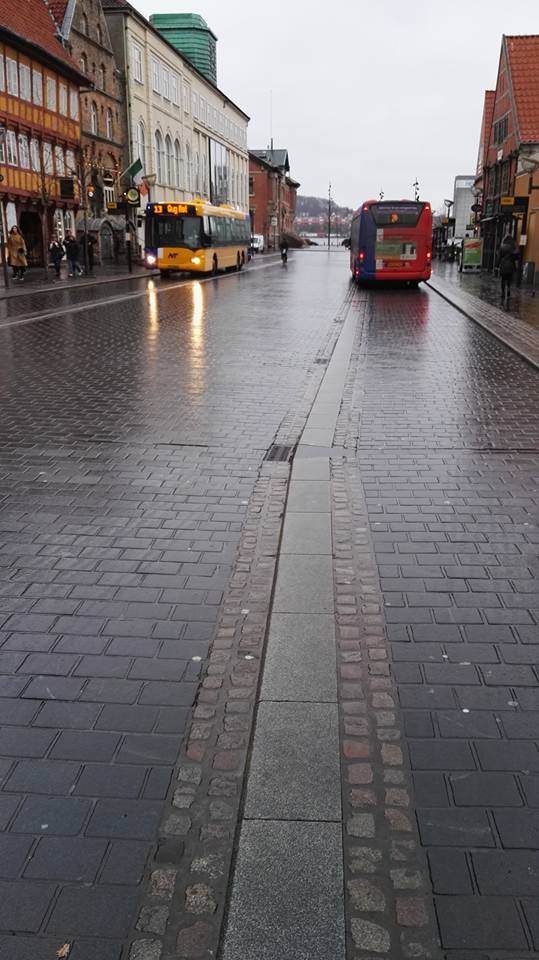
\includegraphics[scale=0.2]{billederogfigur/Busstoppesteder.jpg}
  \end{adjustbox}
   \caption{De to busstoppesteder}
 \end{figure}

På \cref{fig:Busstoppesteder} kan man se de to etablerede busstoppesteder, som er placeret lige efter, hvor Bispensgade udmunder ved Østerågade((henvis til flow kortet)). Placeringen af bustoppestederne er lige udenfor det mest befærdede område, som strækker sig mellem de to gågader og ned ad Nytorv. Placeringen er medvirke til, at det skaber mindst mulige trafikale problemer. Logisk er det også det helt rigtige sted det er placeret, da det reelt set er det eneste sted i området, hvor der er plads til en sådan etablering.
I et Shared Space område kræves også mange holdepladser til cykler. På Nytorv er der på begge sider af vejen et forholdsvist bredt fortov, som har til formål, at skabe en masse plads, hvor cyklerne kan holde parkeret. Det er en nødvendighed, da der færdes mange cykler i området, og for at de mange cyklister skal kunne benytte sig af de mange shopping faciliteter, kræves der altså nogle holdesteder. %((mangler billede af holdepladser))
Der er altså rigtigt mange træk, som man i området kan observere, minder meget om et Shared Space’ princip, og projektet vil i det næste afsnit undersøge, hvordan området bliver benyttet.

\subsection{Trafikanternes benyttelse af Nytorv som et Shared Space}
\label{benyttelse_omrade}
Den ens belægning, den manglende afmærkning og de få skilte kan gøre det svært at orientere sig i Nytorv/Østerågade området. Der er meget få retningslinjer og afmærkning til at lede trafikanterne, hvis stort set ingen.

\begin{figure}[htbp]
   \label{fig:Fodfelt}
   \centering
   \begin{adjustbox}{max width=\textwidth}
     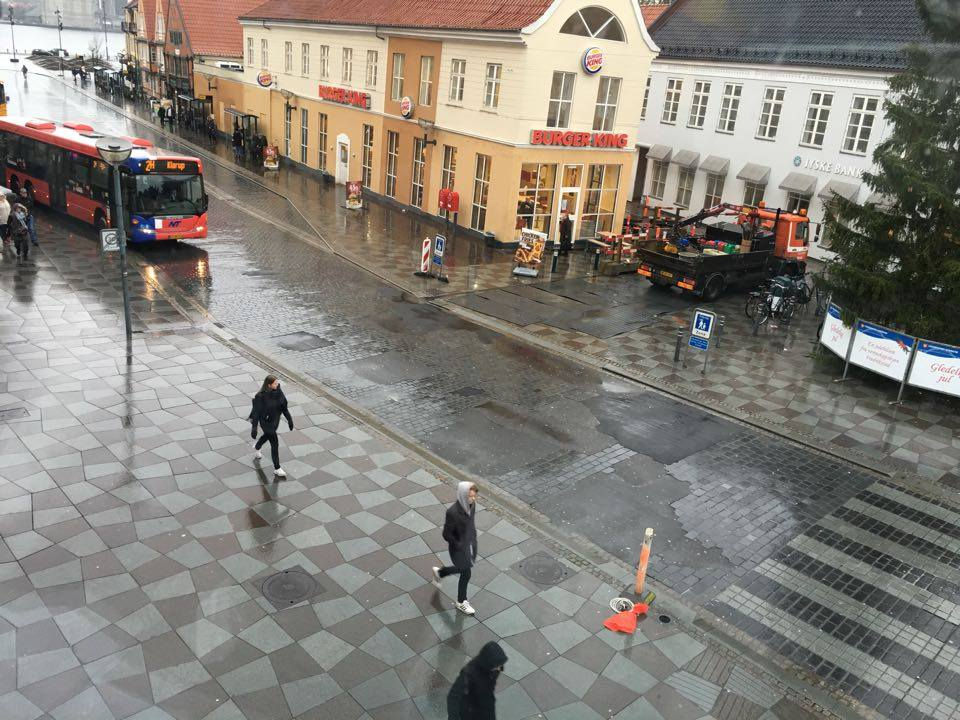
\includegraphics[scale=0.3]{billederogfigur/Fodfelt.jpg}
  \end{adjustbox}
   \caption{Fodgængeroverfeltet}
 \end{figure}

På \cref{fig:Fodfelt} kan man se et af de to fodgængerfelter, som er i området. Det er på billedet let nok at se afmærkningerne, da billedet er taget fra et fugleperspektiv. Men en observation af dette område kan bekræfte, at det kan være svært for cyklisterne at se fodgængerfeltet, når de kommer cyklende mod det. Det er især cyklister, som kommer rundt svinget fra Nytorv mod havnen. Svinget kan ses til venstre i billedet på \cref{fig:Nytorv}. Der skal her nævnes, at fodgængerfeltet er placeret lige efter svinget, så man kan her forestille sig at \cref{fig:Nytorv} og \cref{fig:Fodfelt} hænger sammen. Det er blandt andet også denne hypotese, at interviewsene senere i rapporten tager lidt udgangspunkt i, hvor trygheden for de passerende fodgængere undersøges.
Det er dog langt fra alle fodgængerne der benytter sig af fodgængerfelterne. Der er ikke et fast struktureret trafik flow, som man ved andre områder vil kunne observere. Mange fodgængere passere området midt over torvet, som er det torv, der er illustreret på \cref{fig:Nytorv}. Cyklisterne agerer også meget uensartet, og det er netop en af sideeffekterne ved et Shared Space område. En undersøgelse af trafik flowet i området, vil blive foretaget senere i rapporten. Det er her spørgsmålet kommer ind i billedet, om flere retningslinjer vil skabe mere tryghed, eller et uensartet trafik flow er lige så trygt at færdes i. Det er i hvert fald tydeligt, at der er blevet formået at binde området sammen set fra de bløde trafikanters perspektiv. Udelukkelsen af biler har tydeligt præget fordelingen af trafikantgrupper i området, og langt størstedelen er fodgængere og cyklister. Den balancerende virkning mellem de forskellige trafikantgrupper er også tilstede, og det er ikke et område, hvor man vil forvente en masse ulykker. En vurdering af området tyder på, at den indbyrdes respekt overfor hinanden, mellem de forskellige trafikantgrupper, ikke er pålagt af området, men individet selv, netop fordi, at området ikke pålægger det. Shared Space har altså en form for psykologisk effekt, som får trafikanterne til at være opmærksomme på hinanden, og hjælpe hinanden gennem området bedst muligt. Dog er dette ikke et argument for et trygt område at færdes i. Kvalitative interviews vil her være en god måde at undersøge på, om især fodgængerne føler sig trygge, ved at passere området.
De biler, som på trods af forbuddet, vælger at færdes dernede, kører generelt med en lav hastighed. Det samme er at sige om busserne. De opfylder også oftest kravet om en pålagt respekt overfor de bløde trafikanter, og holder tilbage for fodgængeroverfeltet. I forhold til bustrafikken, må det som antaget, forsinke dem en smule, dog begrænset, da det kun er det ene fodgængerfelt, der skal passeres.
I det næste afsnit vil der blive undersøgt via kvalitative interviews, om fodgængerne føler sig trygge overfor cyklisterne, busserne og bilerne, når de passere fodgængeroverfeltet. Herved også for at få en forståelse af, om den balance Shared Space har til formål, er opfyldt.


<<<<<<< HEAD
=======



>>>>>>> fd7bded0e9130e2abfc03b6c27c49a37aeabe04a
\subsection{Interviews}
Eftersom at fodgængere blev observeret som et problem for cyklisterne, så blev fodgængere også observeret grundigere. Der blev identificeret, at fodgængere også var delvis utryg ved Nytorv området, hvilket gav årsag til grundigere undersøgelse, med blandt andet interview med fodgængere.\footnote{XXXXXXX vej.lovportaler.dk} http://vejregler.lovportaler.dk/showdoc.aspx?t=%2fV1%2fNavigation%2fTillidsmandssystemer%2fVejregler%2fAnlaegsplanlaegning%2fTrafikarealer+by%2fVejgeometri+i+byomrader%2f&docId=vd-shared-space-full 10/11-2015}


\subsection{Anvendelse af interviews i praksis}
I denne rapport blev der foretaget et kvalitativt interview med forbigående fodgængere ved Nytorv/Østerågade i Aalborg. Det kvalitative interview leder til kvalitativ viden fra forskellige aspekter, og virker ofte som en metode for, at undersøge nogle bestemte forholde. Under det kvalitative interview bliver interviewpersonerne opfordret til at beskrive hvad de oplever, føler og hvilke ideer og holdninger de har til det givende emne. Derved opnås der under det kvalitative interview konkret viden, i stedet for generelle meninger, som er karakteristisk ved det kvantitative interview. \footnote{ Hans Reitz Forlag, interview introduktion til et håndværk 2. udgave, side 48}
\\

Herunder kunne et eksempel på en kvalitativ interview være et delvis strukturerede interview, som anvendes, når den teoretisk og praktisk viden er kendt på forhånd, men er åben for nye synsvinkler, holdninger og oplevelser, som interviewpersonerne deler. I forbindelse med interviewet bliver der belyst nogle forholde, som til en vis grad er udarbejdet på forhånd. I rapporten er der en påstand om at det kan føles utrygt, når trafikmiljøet er integreret nede ved Nytorv/Østerågade, herved bruges interviewene blandt andet, som belæg for at det kan virke utrygt, at færdes i området. \footnote{Ib Andersen, Den skinbarlige virkelighed, side 169}


\subsection{Formålene med interviewene ved Nytorv/Østerågade i Aalborg}
Formålet med interviewet er, at finde initierende problemer og løsninger til, hvordan der kan opnås en effektiv og innovativ sammenbinding af gågade systemet i Aalborg Nytorv/Østerågade. Der blev interviewet fodgængere og cykelister, med hensigten om at de skulle have medbestemmelse i, at skabe en bedre oplevelse af sikkerhed og tryghed i området.
\\

I den forbindelse blev der gennemført ca. 20 kvalitative interviews , hvor der blev talte med en forbigående fodgængere og cyklister ad gangen. Interviewene skal bidrage med, at finde løsninger til, hvordan der kan skabes et sikkert og trygt trafikmiljø for alle fodgængere og cyklister.
I værktøjskassen vil der være en række spørgsmål om, hvordan fodgænger og cyklister oplevelser er med at have et integreret trafikmiljø, ønsker ift. hvordan en effektiv sammenbinding af gågadesystemet i Aalborg kunne være, og hvad de tænker om forslaget om løsningerne til problemstillingen i området.
Interviewet er åbent undersøgende om fodgængernes og cyklisterne sikkerhed og tryghed. Der blev afsat 2 timer til interviewet den 14 oktober 2015 fra klokken 13 til 15.\footnote{https://innovation.blogs.ku.dk/metode/det-kvalitative-interview/ 27/10- 2015}

\subsection{Interview resultaterne med forbigående fodgængere og cyklister ved Nytorv/Østerågade i Aalborg}
 Ud fra de kvalitative interviews (se bilag  \cref{chap:interviews}) med forbigående fodgængere og cykelister, resulterede interviewene til, at der var en større enighed om hvorvidt forbipasserende fodgænger og cyklister følte sig utrygge ved at passere Nytorv/Østerågade området i forbindelse med, det integreret trafikmiljø der er. Eksempelvis påstod flere af interviewpersonerne, at de brugte en del tid på at holde øje med om cyklisterne havde set dem. Spørgsmålet lød på om de følte sig trygge ved at gå over fodgængerfeltet, når der færdes mange cyklister ude ved Nytorv/Østerågade i Aalborg, hertil svarede en del,\emph{“Egentlig ikke - jeg synes, at cyklerne kommer meget uventet og meget hurtigt. Jeg holder utroligt meget øje.”} Dette beviser blot at flere fodgængere føler sig utrygge ved at gå over fodgængerfeltet ved området, selvom at de har førsteret til at gå over.
\\

Der er flere årsager, til hvorfor fodgængerene og forbigående cyklister føler sig utrygge i området, eksempelvis mente interviewepersonerne,\emph{”(…), at der kan være kaos herude nogle gange, og det er både cyklister, biler og busser der skaber den kaos.”}. Det vil sige at årsagen til følelsen af utrygheden iblandt fodgængere og forbigående cyklister, delvis er det integreret trafikmiljø der eksisterer, som i visse tilfælde kan udløse et kaos, manglende hensynstagen til andre trafikgrupper, såsom cyklister som ikke holder for fodgængerne ved fodgængerfeltet, mindre kontrol over udelukkelse af privatbiler, da de kan fremføre til større skader, dog er der ingen af interviewpersoner der har oplevet ulykker,  eksempelvis mener en interviewperson, at før vedkommende kan føle sig tryg i trafikken kræver det,\emph{“(…) at busserne og bilerne holder tilbage. Det er dem der kan lave noget skade. Jeg har gået herinde rigtig meget, og jeg har aldrig set en ulykke.”}, selvom at ingen af interviewpersonerne har oplevet en ulykke i området, er tanken om at en større ulykke kan finde sted alligevel skaber utryghed. Derudover skaber den knibende vejplads til cykelister også en utryghed for fodgængerne, eksempelvis påstod en interviewperson, at \emph{“(…) på Boulevarden lagde jeg mærke til at cyklisterne ikke kunne være der, så de måtte trække deres cykler på fortovet (…)".}, da cyklisterne i vissetilfælde trækker deres cykler på fortovet af manglende plads til dem ved Nytorv/Østerågade, skaber det en utryghed for fodgængerne, der går på fortovet.
\\

<<<<<<< HEAD
Der var også en enighed iblandt de forbipasserende fodgængerne og cyklisterne om, at der ønskes en differentiering mellem cyklisterne og kørebanerne. Ønsket lød på, at \emph{“(…) lede cyklerne uden om Nytorv eller dele cyklisterne ud fra kørebanen(…)"}. I og med, hvis ønsket om et differentierede trafikområde blev vedtaget bevæger Nytorv/ Østerågade sig længere væk fra shared space konceptet, hvilket i vissetilfælde vil virke mere trygt for alle trafikantgrupper.
I forbindelse med spørgsmålet om, hvilke ønsker eller forslag de forbigående fodgængere og cykelister havde til at binde gågaden sammen, blev der eksempelvis forslået nogle ønsker om, at \emph{”(…)man kan male fodgængerfeltet hvidt.”}. På nuværende tidspunkt er fodgængerfeltet mellem Bispensgade og Lille Kongensgade grå, en hvid fodgængerfelt frem for den grå, vil virke mere synlig for de kørende og cyklende trafikantgrupper. Nogle interviewpersoner mener også, at mere kontrol over udelukkelse af privatkørsel, en gennemvej for cykelister der skal mod universitet, undergang, overgang eller tunnel vil skabe mere tryghed i området. I den anledning var der også flere ønsker om en køretøjsfrizone, dog var der i højere grad enighed om, at cyklisterne ikke skulle udelukkes fra Nytorv/Østerågade, da nogle synes at de skaber liv i området, og andre påstod at det ikke ville kunne lade sig gøre med den store mængde af cyklister, der cykler til universitet og andre steder hver dag.
=======
Der var også en enighed iblandt de forbipasserende fodgængerne og cyklisterne om, at der ønskes en differentiering mellem cyklisterne og kørebanerne. Ønsket lød på, at \emph{“(…) lede cyklerne uden om Nytorv eller dele cyklisterne ud fra kørebanen(…)"}. I og med, hvis ønsket om et differentierede trafikområde blev vedtaget bevæger Nytorv/ Østerågade sig længere væk fra shared space konceptet, hvilket i vissetilfælde vil virke mere trygt for alle trafikantgrupper. 
I forbindelse med spørgsmålet om, hvilke ønsker eller forslag de forbigående fodgængere og cykelister havde til at binde gågaden sammen, blev der eksempelvis forslået nogle ønsker om, at \emph{”(…)man kan male fodgængerfeltet hvidt.”}. På nuværende tidspunkt er fodgængerfeltet mellem Bispensgade og Lille Kongensgade grå, en hvid fodgængerfelt frem for den grå, vil virke mere synlig for de kørende og cyklende trafikantgrupper. Nogle interviewpersoner mener også, at mere kontrol over udelukkelse af privatkørsel, en gennemvej for cykelister der skal mod universitet, undergang, overgang eller tunnel vil skabe mere tryghed i området. I den anledning var der også flere ønsker om en køretøjsfrizone, dog var der i højere grad enighed om, at cyklisterne ikke skulle udelukkes fra Nytorv/Østerågade, da nogle synes at de skaber liv i området, og andre påstod at det ikke ville kunne lade sig gøre med den store mængde af cyklister, der cykler til universitet og andre steder hver dag. 

\footnote{Fatimah Daoud,æbleskiver}
 



>>>>>>> fd7bded0e9130e2abfc03b6c27c49a37aeabe04a

\section{Trafiktællinger}
\label{sub:trafiktaellinger}
Dette afsnit tager udgangspunkt i kilden:
\\ http://vej08.vd.dk/mastra/mastradok/dok/TrafiktaellingerPlanUdfoerEfterb.pdf

Trafiktællinger udføres til mange formål. Det gælder alt fra at kontrollere den overordnede vejplanlægning til at undersøge klagesager om for høje trafik hastigheder. Trafiktællinger bruges bl.a. til at finde løsninger til opgaver omhandlende trafiksikkerhed, kapacitet og miljøforhold, samt statistikker over trafikudviklingen og hastigheden af vejnettet. Man kan foretager trafiktællinger manuelt eller ved brug af maskiner. 
Manuelle tællinger fungerer ved at personer registrere trafikken på det pågældende sted, ofte ved hjælp af tælleblokke, håndtællere eller håndterminaler. Ved maskine tælling fortages registreringerne automatisk ved brug af et tælleapparat, hvor mennesker ikke medvirker.

\subsection{Manuel tælling}
\label{sub:manuel_taelling}
Manuel tælling er som sagt, hvor det er mennesker der tæller trafikken. Manuel tælling er en god metode, når der ønskes at kende trafikkens specifikke trafikstrømme. Et typisk forløb for manuel tælling er opbygget af 6 trin.
\\\\
1) Som det første skal formålet for tællingen bestemmes, samt hvilken resultat type, som ønskes af opnå.
\\\\
Vores formål med trafiktællingen er tælle hvor mange fodgængere, cykelister og billister som befinder sig inde ved Nytorv og Østerågade. Hvorefter vi vil omregne resultaterne til årsdøgnstrafik ÅDT. Desuden vil vi notere, hvilken retning trafikanten kom fra og hvilken retning trafikanten skal hen, og herved kunne lave et flowkort af trafikken.
\\\\
2) Der skal besluttes placeringen af tælleposterne, hvor der skal tages hensyn til at tælleren ikke genere trafikken. Tællerne skal også have frit udsyn for parkerende biler, buskaser og lignende under hele tælleperioden. Man skal derfor overveje om forholdene kan ændre sig undervejs.For at have et optimalt overblik over tælleområdet, vurderede vi på tælledagen hvor vi bedst kunne placere os uden at generer trafikken og noterer alle trafikanterne. Vi endte med at sidde uden for The Harp som ligger lige ud til Østerågade og på første sal i McDonald’s hvor der var godt overblik af Østerågade og Nytorv.
\\\\
3) En af de betydelige usikkerheder ved trafiktællinger, er valget af tælleperioden. Der kan være meget stor variation fra dag til dag og time til time, hvis man. ønsker at finde årsdøgntrafikken. Der er f.eks. stor forskel på trafikmængden i weekenden kontra hverdage og myldertiden om morgen og eftermiddagen kontra midt på dagen og om aftenen og natten. Manuelle tællinger vare typisk 4, 6 eller 12 timer og sjældent et helt døgn. Vi valgte at lave trafiktællingerne tirsdag d. 24 november kl. 13:00 til 15:00. Vi havde valgt tidspunktet ud fra hvornår vi havde tid i forhold til vores skema, og vi vurderede at det er omkring dette tidspunkt på dagen hvor der er flest mennesker i området, eftersom at der ligger mange butikker i nærheden.
\\\\
4) Når tælleposterne og tidspunkterne er fastlagt, bestemmes antallet af tællere til posterne, efter trafikmængden ved stedet. Ifølge vejdirektoratet er kvaliteten af resultaterne afhænger af antal tællere. Er tælleposterne underbemandet, vil resultaterne blive uanvendelige. Hvis man er uvidende om trafikmængden, og dermed antallet af tæller som er nødvendige, kan man foretage en prøvetælling inden.

\begin{figure}[htbp]
   \label{fig:taellingstype}
   \centering
   \begin{adjustbox}{max width=\textwidth}
     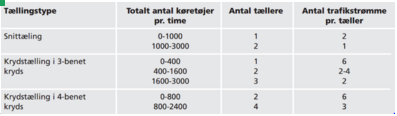
\includegraphics[scale=1]{billederogfigur/taellingstype.jpg}
  \end{adjustbox}
   \caption{Tællingstyper}
 \end{figure}
 
 \begin{figure}[htbp]
   \label{fig:krydstaelling}
   \centering
   \begin{adjustbox}{max width=\textwidth}
     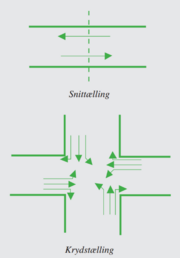
\includegraphics[scale=1]{billederogfigur/krydstaelling.jpg}
  \end{adjustbox}
   \caption{Skitse af krydstælling}
 \end{figure}
 
Der skal også bestemmes valget af tælleudstyr. Ved mindre trafikmængder kan der anvendes blyant og papir, ved stører trafikmængder anvendes ofte håndtællere, håndterminaler eller tællepulte. Da der er mange trafikanter i området og vi alle er uerfarne med trafiktællinger, har vi valgt at vi alle 6 i gruppen skal ud og tælle. Vi har valgt at lave et tælleskema i Excel, som vi printer ud i papir og kan afkrydse vores talte trafikanter i.
\\\\
5) Inden tællerne begynder, er det vigtigt at de er sat sig ind i overstående bestemmelser for tælleforløbet, således der ikke opstår tvivler undervejs. Ligeledes udarbejdes et tælleskema inden tællingen påbegyndes. 
\\\\
6) Resultatbehandling af tællingen. 
Der skal også bestemmes valget af tælleudstyr. Ved mindre trafikmængder kan der anvendes blyant og papir, ved stører trafikmængder anvendes ofte håndtællere, håndterminaler eller tællepulte.
Da der er mange trafikanter i området og vi alle er uerfarne med trafiktællinger, har vi valgt at vi alle 6 i gruppen skal ud og tælle. Vi har valgt at lave et tælleskema i Excel, som vi printer ud i papir og kan afkrydse vores talte trafikanter i.
 
\begin{figure}[htbp]
   \label{fig:trafiktaellingen}
   \centering
   \begin{adjustbox}{max width=\textwidth}
     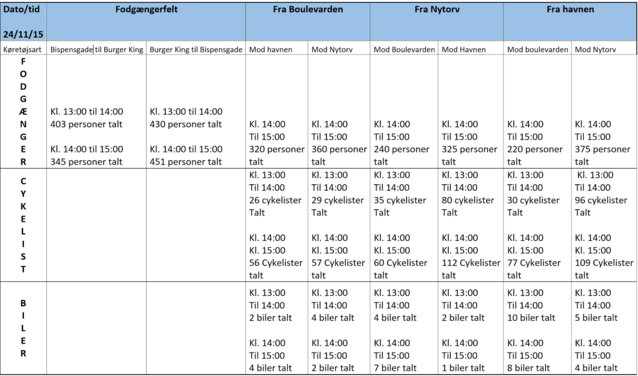
\includegraphics[scale=1]{billederogfigur/trafiktaellingen.jpg}
  \end{adjustbox}
   \caption{Resultat af trafiktælling}
 \end{figure}
Der findes ingen omregningsfaktor af fodgængere til ÅDT, derfor har vi vurderet vores tælling, ud fra forholdende på tælledagen. Vi noterede 2636 fodgængere tirsdag den 24 november Kl. 14:00 til 15:00. På dette tidspunkt har skole og gymnasieelever måske fået fri, mens alle som har et 8 til 16 job stadig er på arbejde. Derfor ville der måske være flere hvis tællingen var taget senere. Til gengæld hvis tællingerne var taget tidligere og midt i skoletiden ville antallet af fodgængere nok være mindre. En anden faktor er, at det regnede mens vi talte. Vi tror at regnvejret vil holde mange indendørs og vente til en anden dag med at shoppe i midtbyen. Desuden har dagen og årstiden en stor indflydelse på antallet af fodgængere på Nytorv og Østerågade. Eftersom at der er mange butikker i området, er det ikke bolig – arbejde trafik som kommer her. Det er nærmere folk, med et ærinde som f.eks. at shoppe eller at gå på café. Derfor kunne man forestille sig at der vil komme flere mennesker i weekenden hvor folk har fri for arbejde end i hverdagen. I sommerferien vil man også kunne finde meget mere liv, fordi folk mødes, og der bliver afholdt diverse arrangementer nede i byen. Hvis vi skal konkludere på usikkerhederne, er antallet af fodgængere i Østerågade og Nytorv meget situations afhængig. Det vil være stor forskel på en varm dag i sommerferien hvor byen tiltrækker med faciliteter og arrangementer og en kold regnvejrsdag i efteråret.

\subsection{Opregning af trafiktællinger til ÅDT}
\label{sub:opregning}
Ved at opregne et antal talte cykler og biler på én dag til ÅDT, vil der altid være en usikkerhed. 
I følgende resultatbehandling vil der være fokus på en trafiktælling af cykler og biler ved Nytorv i Aalborg tirsdag d. 24/11 i tidsrummet 14-18. I dette tidsrum er der tale om en blanding af såkaldt bolig/arbejde og by/lokal trafik, da det er i dette tidspunkt, at gennemsnittet af befolkningen får fri fra arbejde og skole, går på indkøb, og i dette tidsrum, at folk skal hjem til sig selv.
Antallet af biler, som vi fik talt i perioden var 104, og antallet af cykler i samme periode var 1408.
For at opregne en trafiktælling, som denne til årsdøgnstrafik, skal man bruge en bestemt formel:
$$ T \times FDT \times FUHDT \times FUDT \times FÅDT = ÅDT $$ eller $$ UDT \times FÅDT = ÅDT$$ , hvor:

$$T = Talt trafik$$

$$UDT = Ugedøgstrafik$$

$$FDT = Opregningsfaktor til døgntrafik i tælleugen$$

$$FUHDT = Opregningsfaktor til ugehverdagsdøgntrafik i tælleugen$$

$$FUDT = Opregningsfaktor til ugedøgntrafik i tælleugen$$

$$FÅDT = Opregningsfaktor til årsdøgntrafik i tælleåret$$ 

$$FÅR = Opregningsfaktor fra tælleår til andet år$$

Tallene aflæses i skemaerne på side 102-117. Den sidstnævnte formel til at udregne ÅDT’en, er den mest oplagte, da der findes en nem metode at finde frem til UDT, og hernæst skal FÅDT blot aflæses og ganges med UDT, for at vi kan finde ÅDT.

\subsection{ÅDT}
\label{AEDT}
\subsubsection{Cyklernes samlede ÅDT på Nytorv i Aalborg}
$$DT = T \times FDT = 1408 \times 1/(0,083+0,106+0,098+0,065) = 4.000$$
$$UHDT = DT \times FUHDT = 4.000 \times 0,95 = 3.800$$
$$UDT = UHDT \times FUDT = 3.800 \times 0,81 = 3.078$$
$$ÅDT = UDT \times FÅDT = 3.078 \times 1,15 = 3.540$$
\subsubsection{ÅDT for cykler fra Boulevarden mod Havnen}
$$DT = T \times FDT = 162 \times 1/(0,083+0,106+0,098+0,065) = 460 $$
$$UHDT = DT \times FUHDT = 460 \times 0,95 = 437$$
$$UDT = UHDT \times FUDT = 437 \times 0,81 = 354$$
$$ÅDT = UDT \times FÅDT = 354 \times 1,15 = 407$$
\subsubsection{ÅDT for cykler fra Boulevarden mod Nytorv}
$$DT = T \times FDT = 172 \times 1/(0,083+0,106+0,098+0,065) = 489$$
$$UHDT = DT \times FUHDT = 489 \times 0,95 = 465$$
$$UDT = UHDT \times FUDT = 465 \times 0,81 = 377$$
$$ÅDT = UDT \times FÅDT = 377 \times 1,15 = 434$$
\subsubsection{ÅDT for cykler fra Nytorv mod Boulevarden}
$$DT = T \times FDT = 176 \times 1/(0,083+0,106+0,098+0,065) = 500$$
$$UHDT = DT \times FUHDT = 500 \times 0,95 = 475$$
$$UDT = UHDT \times FUDT = 475 \times 0,81 = 385$$
$$ÅDT = UDT \times FÅDT = 385 \times 1,15 = 443$$
\subsubsection{ÅDT for cykler fra Nytorv mod Nytorv}
$$DT = T \times FDT = 286 \times 1/(0,083+0,106+0,098+0,065) = 813$$
$$UHDT = DT \times FUHDT = 813 \times 0,95 = 772$$
$$UDT = UHDT \times FUDT = 772 \times 0,81 = 625$$
$$ÅDT = UDT \times FÅDT = 625 \times 1,15 = 719$$
\subsubsection{ÅDT for cykler fra Havnen mod Boulevarden}
$$DT = T \times FDT = 224 \times 1/(0,083+0,106+0,098+0,065) = 636$$
$$UHDT = DT \times FUHDT = 636 \times 0,95 = 604$$
$$UDT = UHDT \times FUDT = 604 \times 0,81 = 489$$
$$ÅDT = UDT \times FÅDT = 489 \times 1,15 = 562$$
\subsubsection{ÅDT for cykler fra Havnen mod Nytorv}
$$DT = T \times FDT = 388 \times 1/(0,083+0,106+0,098+0,065) = 1.102$$
$$UHDT = DT \times FUHDT = 1.102 \times 0,95 = 1.047$$
$$UDT = UHDT \times FUDT = 1.047 \times 0,81 = 848$$ 
$$ÅDT = UDT \times FÅDT = 848 \times 1,15 = 975$$
\subsubsection{Bilernes samlede ÅDT på Nytorv i Aalborg}
$$DT = T \times FDT = 216 \times 1/(0,068+0,091+0,095+0,073) = 661$$
$$UHDT = DT \times FUHDT = 661 \times 1,02 = 674$$
$$UDT = UHDT \times FUDT = 674 \times 0,91 = 613$$
$$ÅDT = UDT \times FÅDT = 613 \times 1,00 = 613$$
\subsubsection{ÅDT for biler fra Boulevarden mod Havnen}
$$DT = T \times FDT = 24 \times 1/(0,068+0,091+0,095+0,073) = 73$$
$$UHDT = DT \times FUHDT = 73 \times 1,02 = 74$$
$$UDT = UHDT \times FUDT = 74 \times 0,91 = 67$$
$$ÅDT = UDT \times FÅDT = 67 \times 1,00 = 67$$
\subsubsection{ÅDT for biler fra Boulevarden mod Nytorv}
$$DT = T \times FDT = 24 \times 1/(0,068+0,091+0,095+0,073) = 73$$
$$UHDT = DT \times FUHDT = 73 \times 1,02 = 74$$
$$UDT = UHDT \times FUDT = 74 \times 0,91 = 67$$
$$ÅDT = UDT \times FÅDT = 67 \times 1,00 = 67$$
\subsubsection{ÅDT for biler fra Nytorv mod Boulevarden}
$$DT = T \times FDT = 44 \times 1/(0,068+0,091+0,095+0,073) = 135$$
$$UHDT = DT \times FUHDT = 135 \times 1,02 = 138$$
$$UDT = UHDT \times FUDT = 138 \times 0,91 = 126$$
$$ÅDT = UDT \times FÅDT = 126 \times 1,00 = 126$$
\subsubsection{ÅDT for biler fra Nytorv mod Havnen}
$$DT = T \times FDT = 12 \times* 1/(0,068+0,091+0,095+0,073) = 37$$
$$UHDT = DT \times FUHDT = 37 \times 1,02 = 38$$
$$UDT = UHDT \times FUDT = 38 \times 0,91 = 35$$
$$ÅDT = UDT \times FÅDT = 35 \times 1,00 = 35$$
\subsubsection{ÅDT for biler fra Havnen mod Boulevarden}
$$DT = T \times FDT = 76 \times 1/(0,068+0,091+0,095+0,073) = 232$$
$$UHDT = DT \times FUHDT = 232 \times 1,02 = 237$$
$$UDT = UHDT \times FUDT = 237 \times 0,91 = 216$$
$$ÅDT = UDT \times FÅDT = 216 \times 1,00 = 216$$
\subsubsection{ÅDT for biler fra Havnen mod Nytorv}
$$DT = T \times FDT = 36 \times 1/(0,068+0,091+0,095+0,073) = 110$$
$$UHDT = DT \times FUHDT = 110 \times 1,02 = 112$$
$$UDT = UHDT \times FUDT = 112 \times 0,91 = 102$$
$$ÅDT = UDT \times FÅDT = 102 \times 1,00 = 102$$















\subsection{Første observation}
\label{sub:foerste_obs}
Aalborg er byen som arbejder på, at skabe en cykelby.%(http://www.aalborgcykelby.dk/aalborg-cykelby)
Som en cykelby kræver det, at der er en optimal sikkerhed for cyklister blandt andre trafikantgrupper. Trafik Flowet ved åbningen af Nytorv blev observeret, området ved McDonalds og Burger King, hvor der kunne ses at de fleste cyklister havde nogle mindre alvorlige konflikter med bilerne der krydser Nytorv illegalt. Tværtimod havde cyklisterne lidt større konflikter med fodgængere samt busserne, hvilket også gav et stop for trafikflowet. Derudover kunne der ikke observeres en tryghed på cyklisternes ansigtsudtryk, eftersom de hele tiden skulle være fokuseret og parat til, at bremse ned for fodgængere eller busser. En mindre vurdering kunne bekræfte, at cyklisterne ikke havde en optimal tryghed ved området pga. fodgængere og delvist busserne, eftersom busserne ikke hele tiden krydser Nytorv, men blot hver 5.-6. minut.

Trafik flowet ved slutningen af Nytorv blev observeret, området ved Salling og Friis, her kunne der ses konflikter blandt bilister og cyklister, eftersom cyklisternes cykelsti bliver fjernet. Der kunne tydelig ses en utryghed blandt cyklisterne og bilisterne, da trafikantgrupperne delte vejbanen, hvilket skabte ustruktureret trafikflow ved området og nogle ulovlige overhalinger.

Eftersom fodgængere blev observeret som et problem for cyklisterne, så blev fodgængere også observeret grundigere. Der blev identificeret, at fodgængere også var delvis utryg ved Nytorv området, hvilket gav årsag til grundigere undersøgelse, såsom interview med fodgængere.

\subsection{Dybbere undersøgelse af første observation}
\label{sub:dyb_undersoelse}
I første omgang blev der blot observaret, hvor der blev antaget en række antagelser. Hvoraf der til næste observation blev gjort brug af mere specifikke metoder for at identificere trygheden på Nytorv området i Aalborg.
\\\\
Metoderne bag næste observation var, at identificere konflikter ved området. Ved hjælp af konflikterne kan trygheden og sikkerheden for de forskellige trafikantgrupper identificeres. Inden metoderne bliver præsenteret vil begrebet konflikt defineres først. Begrebet konflikt, er et meget vidt begreb og dækker indenfor flere fagområder,1 men i denne rapport, bliver der nærmere undersøgt for begrebet indenfor vej og trafik. Som umiddelbart vil man definere konflikt, som sammenstød mellem to trafikkanter, men dog udelukker den svenske trafikteknik denne påstand.%Kilde
En af metoderne som bliver anvendt til identificering af konflikterne er den svenske traftikteknik, hvilket er årsagen til deres definition af konflikt bliver brugt i dette projekt.
\\\\
Den svenske trafikteknik beskriver en konflikt mellem to trafikkanter, som har kollisionskurs og vil kolligere, hvis en af trafikkanterne ikke foretager sig en pludselig reaktion for, at forhindre kollisionen.2 Det vil sige, at sålænge et uheld (sammenstød) kan undgås af mindst en af trafikanterne, så vil der være tale om en konflikt. Ved hjælp af den svenske trafikteknik, kan man dele en konflikt i flere grad. De forskellige konfliktgrad er defineret som, alvorlige konflikter, mindre alvorlige konflikter og potentielle konflikter, som også kan ses på \cref{fig:indellingkonflikter} :
 \begin{figure}[htbp]
   \label{fig:indellingkonflikter}
   \centering
   \begin{adjustbox}{max width=\textwidth}
     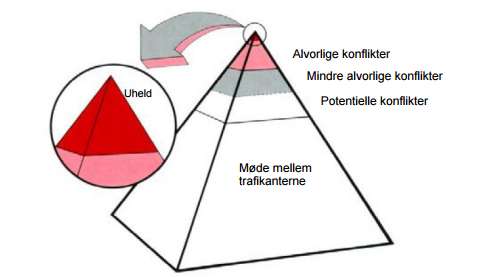
\includegraphics{billederogfigur/konflikt.png} %http://www.trafitec.dk/sites/default/files/publications/konfliktteknikstudier%20i%20kbh%20bykryds.pdf
  \end{adjustbox}
   \caption{Inddeling af konflikter}
 \end{figure}
\newpage

 En konfliktgrad bestemmes ved hjælp af TU-værdi. TU-værdi er defineret som Tid til Ulykke eller også kaldes det TA, altså Time to Accident. Metoden bag bestemmelse af TU-værdien gøres ved hjælp af følgende formel:
 \begin{equation}
  TU=d/V
\end{equation}
Hvoraf TU beskriver tid til ulykke \\ d, beskriver distancen til tænkt kollisionspunkt \\ og V, er hastigheden i den undvigeøjeblik.

Formelen fortæller om forholdet mellem distancen, til det potentielle punkt i en kollision og hastigheden når en af trafikanterne undviger uheldet. Heraf kan der ved hjælp af \cref{fig:tugraff}, ses om konfliktet er alvorlig eller ej.
~\\\\

\begin{figure}[htbp]
  \label{fig:tugraff}
  \centering
  \begin{adjustbox}{max width=\textwidth}
    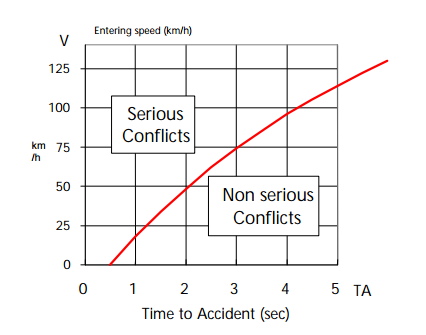
\includegraphics{billederogfigur/tugraf.png} %http://www.tft.lth.se/fileadmin/tft/video_in_traffic/Swedish_conflict_technique.pdf
 \end{adjustbox}
  \caption{TU-graf}
\end{figure}

Som der kan ses på \cref{fig:tugraff}, så er alvorligheden af en konflikt afhængig af både distance samt hastighed, dog har hastighed en større rolle, i tilfælde af hastigheden er høj.
Som udgangspunkt i TU-grafen kan der ses, at en TU værdi over 0.5 ses som ikke alvorlig konflikt, hvorimod en TU værdi under ca. 0.5, vil være en alvorlig konflikt.




For at kunne beregne TA-værdi skal distance og hastighed kendes. Distance og hastighed kan identificeres ved blot nogle målinger ved området, hvilket i dette projekt blev gjort, som ses på \cref{fig:maalingerfrabegge}
\\\\
Som der kan ses på \cref{fig:maalingerfrabegge}, blev området i første omgang målt op fra kanten som er markeret med farven rød til fodgængere feltet og det samme fra den anden kant som er markeret med farven blåt. Bemærk de andre markeringer er forskellige dimensioner som bruges til beregning af TA-værdien, altså i TA-værdi formlen: $$ TU=\frac{d}{V} $$
\begin{figure}
\centering
\begin{subfigure}{1\textwidth}
  \centering
  \includegraphics[width=1\linewidth]{billederogfigur/rodmarkering.jpg}
  \caption{A: Måling fra den højre kant}
  \label{fig:obsomrrod}
\end{subfigure}
\begin{subfigure}{1\textwidth}
  \centering
  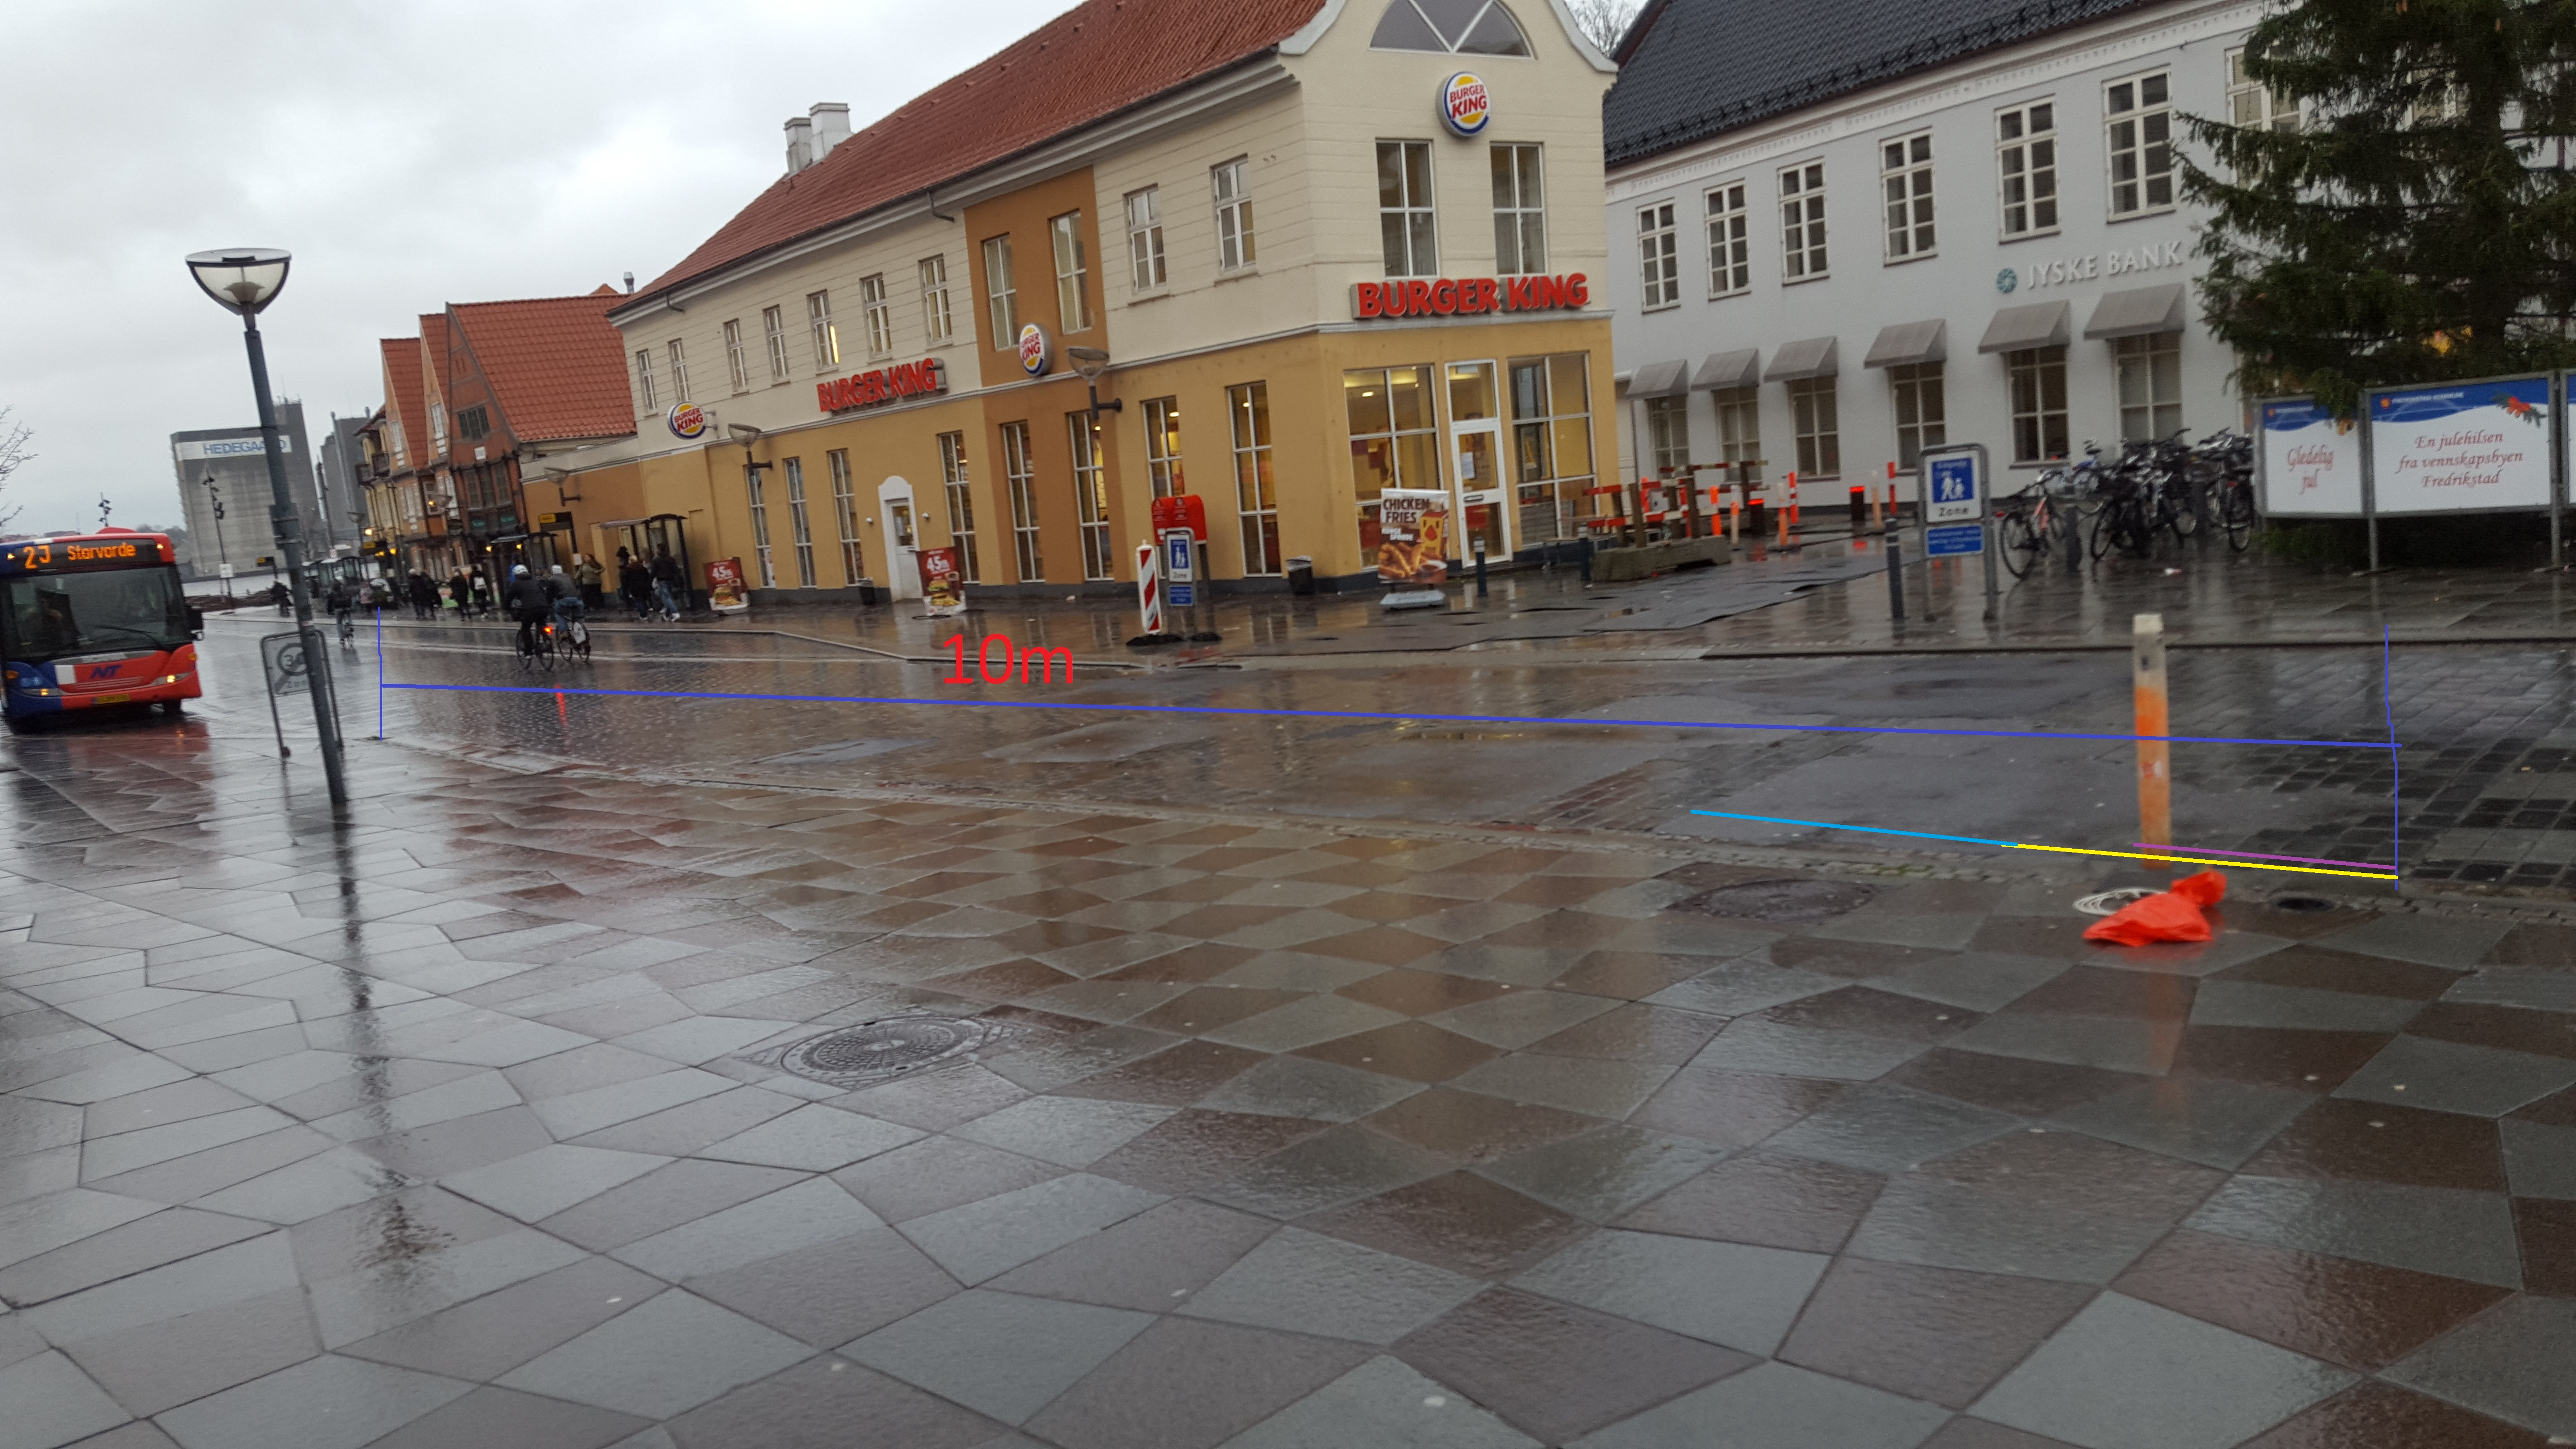
\includegraphics[width=1\linewidth]{billederogfigur/blaamarkering.jpg}
  \caption{B: Måling fra den venstre kant}
  \label{fig:obsomrblaa}
\end{subfigure}
\caption{Målinger fra begge sider}
\label{fig:maalingerfrabegge}
\end{figure}
Herefter var metoden bag TA-værdi, at der blev lavet nogle målinger, dog blev de forskellige distancer noteret og derudover blev der også taget tid til hver enkelt konflikt.
Starttidspunkt: 13:00
\\
Sluttidspunkt:
\\
Placering: Fodgængerfeltet ved Bispengade
\\
Observationssted: Guiness Bar udenfor
\\
Anvendt materiale: Computer og tidsfornemmelse, stopur
\\
Fejlkilder: Regnvejrsdag, egen tidsfornemmelse
\\
Afstand fra havn til fodgængerfelt, som blev brugt til at måle hastighed: 10m
\\
Afstand fra Jyske bank til fodgængerfelt: 10m
\\\\
I første omgang blev tiderne af TA-værdi antaget, som vises i tabellen:
\\\\
\begin{tabular}{ |p{1cm}|p{4cm}|p{4cm}|p{4cm}|  }
\hline
\multicolumn{4}{|c|}{Antaget TA-værdier} \\
\hline
Cykel & Hastighed [km/t] & TA-værdi [s] & Distance [m] \\
\hline
1 & 6   & 1.5 & 2 \\
2 & 10  & 0.7 & 0.5 \\
3 & 4.6 & 1.5 & 2 \\
4 & 11  & 0.4 & 1 \\
5 & 10  & 1 & 2 \\
6 & 9   & 0.1 & 0.5 \\
7 & 12  & 0.6 & 0.5 \\
8 & 10  & 0.7 & 1 \\
9 & 14  & 0.4 & 0.5 \\
10 & 8  & 1   & 2 \\
11 & 12 &0.3  &  1 \\
12 & 11 & 0.6 &   2\\
13 & 10 & 0.8 & 1\\
14 & 6  & 1   & 2\\
15 & 9  & 0.9 & 1\\
16 & 10 & 0.5 & 1\\
17 & 14 & 0.3 &0.5\\
18 & 12 & 0.6 & 0.5\\
19 & 7  & 1 & 2\\
20 & 5  & 1.5 & 2\\
\hline
\end{tabular}




\subsection{Resultater af observation}
\label{sub:def_konflikt}

Som tidligere nævnt, så blev distancen for hvert konflikt noteret, hvilket gøre det muligt at beregne en mere præcis TA-værdi. Tabel X, viser den beregnede TA-værdi for den bestemt hastighed samt distance som blev målt under udførelsen af metoden.
\begin{tabular}{ |p{1cm}|p{4cm}|p{4cm}|p{4cm}|  }
\hline
\multicolumn{4}{|c|}{Beregnet TA-værdier} \\
\hline
Cykel & Hastighed [m/s] & TA-værdi [s] & Distance [m] \\
\hline
1 & 1.6   & 1.25 & 2 \\
2 & 2.8 & 0.1 & 0.5 \\
3 & 1.3 & 1.5 & 2 \\
4 & 3  & 0.3 & 1 \\
5 & 2.8  & 0.7 & 2 \\
6 & 2.5   & 0.2 & 0.5 \\
7 & 3.3  & 0.1 & 0.5 \\
8 & 2.8  & 0.3 & 1 \\
9 & 3.9  & 0.1 & 0.5 \\
10 & 2.2  & 0.9   & 2 \\
11 & 3.3 & 0.3 &  1 \\
12 & 3.1 & 0.6 &   2\\
13 & 2.8 & 0.3 & 1\\
14 & 1.6  & 1.25   & 2\\
15 & 2.5  & 0.4 & 1\\
16 & 2.8 & 0.3 & 1\\
17 & 3.9 & 0.13 &0.5\\
18 & 3.3 & 0.1 & 0.5\\
19 & 1.9  & 1 & 2\\
20 & 1.4  & 1.4 & 2\\
\hline
\end{tabular}


Som beskrevet i afsnit \cref{sub:def_konflikt}, så kan grafen for TA-værdi bruges til, at identificere om hvor alvorlig konflikterne egentlig er ved området. I grafen kan der ses, hvor de beregnede TA-værdier er placeret, altså om det tilhører alvorlig konflikt eller ej.
!!(GRAF skal laves, hvor der er en tildeling af konfliktgraderne, herunder skal beregnede TA-værdier sættes ind)!!
Som der kan ses på grafen, så er størst delen af konflikterne ret alvorlige eftersom, trafikanterne kommer ret tætte på hinanden i nogle bestemte hastigheder.
\\\\
Mens den svenske trafikteknik blev udført ved området, blev der også udført adfærdsregistering ved området. Metoden bag adfærdsregistering vil blive introduceret inden, udførselen bliver præsenteret.
Når	man	vil	observere	nogle	konflikter	mellem	to	eller	flere	forskellige trafikantgrupper,	må	man	lave	nogle	antagelser	om,	hvad	der	egentlig	vil	føre	til	en konflikt.	Man	må	altså	på	forhånd	opstille	nogle	hypoteser,	som	man	via	nogle undersøgelsesspørgsmål,	kan	bruge	til	at	forudse	nogle	formåede	konflikter	mellem nogle	bestemte	trafikantgrupper.	Baggrunden	for	denne	måde	at	undersøge konflikter	på ligger	i,	at	man	sjældent	vil	have	mulighed	for	at	observere	selve konflikterne	eller	uheldene,	da	det	ikke	vil	være	dagligdag	på	det	givne observationssted.	I	denne	undersøgelse	om	fodgængernes	tryghed	på	Nytorv,	vil man altså	ikke	på	observationsdagen	formode,	at	man direkte	vil	observere en alvorlig	konflikt	eller	et	uheld	mellem	en	fodgænger	og	en	cyklist.	Måden	man derimod	vil	kunne	undersøge	de	opstillede	hypoteser	på	og	bygge	sine	spørgsmål	op omkring,	vil	være	at	bruge	en	evalueringsmetode,	hvor	man	kigger	på adfærdsstudier.i Her	fokuserer	man	på	den	typiske	normale	adfærd	på	sit observationssted, og	det	skal	så	underbygge	hypoteserne. Hele	ideen	bag	denne evalueringsmetode	er	at	”forcere indhentningen	af	data”	(samme	kilde),	altså	at forudsige	data	som	belæg	for	sine	antagelser.
I	denne	undersøgelse	vil	adfærdsregistreringen	blive	bygget	op	omkring	figur	(Figur
3	i	det	udleverede	litteratur),	hvor	fokus	ligger	på	dels	ankomsten	mellem
fodgængere	og	cyklister	og	dels	ankomsten	mellem	fodgængere	og	biler på
observationsstedet. Udgangspunktet	herfra	er	så	at	undersøge,	om	der	i	samtidige
ankomster	er	et	tidligt	samspil	eller	et	sent	samspil	mellem	de	to	trafikanter.
Herefter	vurdere,	om	hændelsen ud	fra	de	to	parametre	gik	godt,	om	der	opstod	en
konflikt	eller	der	decideret	skete	et	uheld.	Hypotesen	er	så,	at	hvis	antallet	af	tidlige
samspil	stiger	og	antallet	af	sene	samspil	falder,	så	vil	trafiksikkerheden,	og	derved
trygheden,	blive	forøget.
\begin{figure}[htbp]
  \label{fig:adfreg}
  \centering
  \begin{adjustbox}{max width=\textwidth}
    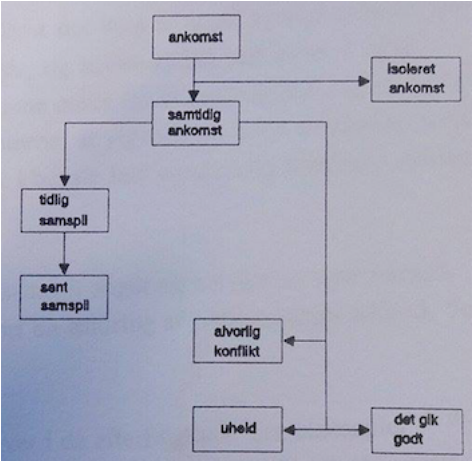
\includegraphics[scale=0.7]{billederogfigur/adfaerdsreg.png} %papir fra vejledern
 \end{adjustbox}
  \caption{Adfærdsregistrering}
\end{figure}
\\\
\subsection{Adfærdsregistrering}
\label{sub:adfregis}

Dette	afsnit	er	inspireret	af	kilden	Konfliktteknik	og	adfærdsstudier.
\\
For	at	kunne	registrere	den	typiske	normale	adfærd	ud	fra	figuren,	er	det	vigtigt	at definere	de	forskellige	begreber. I	tabel	(??)	kan	man	se	en	opdeling	af	de	forskellige	begreber,	en	definition	af	dem og	en	optælling	af	de	forskellige	tilfælde.	Alle	tilfældene	finder	sted	i	en	samtidig ankomst,	da	der	i	en	isoleret	ankomst	ikke	vil	kunne	opstå	en	konflikt	mellem	to parter.	En	samtidig	ankomst	er	i	vores	undersøgelse	defineret	som	cyklisten	eller bilens	ankomst	”til	konfliktpunktet	mindre	end	2.5	sek	efter	eller	mindre	end		1.0	sek	før	fodgængeren.” (kilde udleveret	litteratur)	Ligeledes	skal	cyklen	eller	bilen ikke	være	påvirket	af	andre	parter.	De	skal	altså	være	fritkørende.	Definitionen	på en	fritkørende	bil	eller	cyklist	vil	være,	at	de	ikke	er	styret	af	nogle	forankørende eller	tæt	bagvedkørende,	som	eventuelt	ville	kunne	påvirke fart	og	opmærksomhed.
\\\\
\begin{figure}[htbp]
  \label{fig:adfregtabel}
  \centering
  \begin{adjustbox}{max width=\textwidth}
    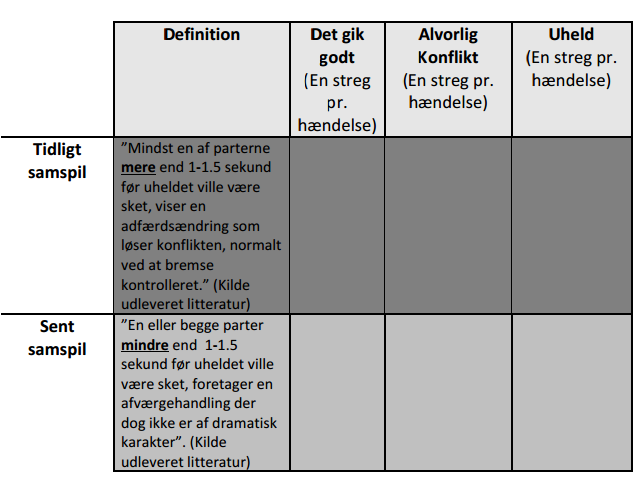
\includegraphics{billederogfigur/obstabel.png} %papir fra vejledern
 \end{adjustbox}
  \caption{Adfærdsregistreringstabel}
\end{figure}
\\\\
\textbf{"Det	gik	godt"} er	defineret	som	en	passering	af	konfliktpunktet,	hvor	situationen
har	været	under	kontrol	og	der	har	været	afstand	mellem	parterne.
8
\\\\
\textbf{"Alvorlig konflikt"}	er	defineret	ud	af	en	afværgehandling,	som	ville	have	ført	til	en
kollision	mellem	to	parter. Afværgehandlingen	sker	inden	for	1-1.5	sekund	før	den
mulige	kollision%(udleveret	litteratur).

\\\\
\textbf{"Uheld"} er	defineret	ved	en	kollision	mellem	to	parter.

Bemærk ved udførselen af denne metode, så blev der set bort fra isolerede ankomster, eftersom det ikke havde meget at sige til undersøgelsen. Herefter blev målingerne fra TA-værdi brugt, hvilket kan ses på \cref{fig:maalingerfrabegge} og alt andet ved observation er det samme som det forrige \cref{sub:dyb_undersoelse}, hvor TA-væriden blev under søgt.
\\
Det blev taget tid for hver reaktion for konflikt, således der kunne identificeres om der var sensamspil eller tidlig. Derudover blev der også set om konflikten gik godt eller om der var tale om alvorlig konflikt, som er defineret som sensamspil. De opnåede resultater kan ses på \cref{fig:adfregtabelresult}.


Resultaterne fra TA-værdi og adfærdsregistering sættes sammen:
\begin{figure}[htbp]
  \label{fig:adfregtabelresult}
  \centering
  \begin{adjustbox}{max width=\textwidth}
    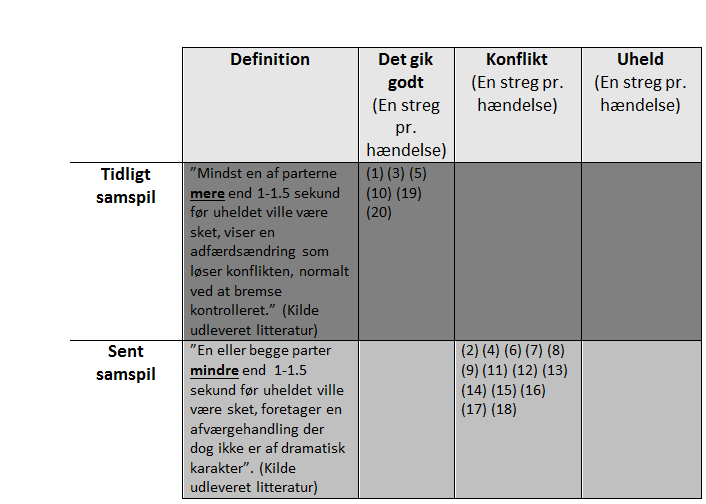
\includegraphics{billederogfigur/obstabelresult.png} %papir fra vejledern
 \end{adjustbox}
  \caption{Adfærdsregistreringstabel med resultater}
\end{figure}

Der var en hypotese om, at hvis antallet af tidlige samspil stiger og antallet af sene samspil falder. så vil trafiksikkerheden og trygheden fra området blive forøget. Ses der på adfærdsregistering \cref{fig:adfregtabelresult}, så kan der observeres at resultaterne er det omvendte af hypotesen, så det vil sige at sikkerheden samt trygheden bliver reduceret ved området. Udefra TA-værdien kunne der også bekræftes, at sikkerheden og trygheden ikke er helt optimalt.
Udefra TA-grafen, så kan der ses, at 7 ud af 20 konflikter ikke er alvorlige, hvoraf 13 ud af 20 er alvorlige. Det svar til, at 65 procent af konflikterne er alvorlige, hvoraf resterne 35 procent er mindre alvorlige som ikke har det stor betydning ved områdets sikkerhed.

